\documentclass{article}

\PassOptionsToPackage{numbers, compress}{natbib}
\usepackage{neurips_2026}

\usepackage[utf8]{inputenc}
\usepackage[T1]{fontenc}
\usepackage{hyperref}
\usepackage{url}
\usepackage{booktabs}
\usepackage{amsfonts}
\usepackage{amsmath}
\usepackage{amssymb}
\usepackage{nicefrac}
\usepackage{microtype}
\usepackage{xcolor}
\usepackage{graphicx}
\usepackage{array}

\graphicspath{{../figures/}}

\title{Cognition-on-Engine: Unlocking Geometric Intuition in LLMs Through Domain-Specific Simulators}

\author{%
  Anonymous Authors \\
  Paper under double-blind review \\
}

\begin{document}

\maketitle

\begin{abstract}
Large language models struggle with geometric reasoning---the visual, kinesthetic, and counterfactual core of low-dimensional intuition. Existing remedies hand the model a generic code interpreter (ToRA, PAL) or train geometry-specialised models (AlphaGeometry); neither is grounded in how human geometric cognition is structured. We propose Cognition-on-Engine (CoE), a framework that pairs an unmodified LLM with a domain-specific engine exposing three cognitive primitives: R (relational structure), T (transformation traces), and C (contrastive counterfactuals). In head-to-head comparison with existing methods (Table~\ref{tab:methods}), CoE scores 3.75/4.0 vs.\ 2.42 for CoT+Code and 1.88 for chain-of-thought; on the main $2^3$ ablation (Table~\ref{tab:full-results}; the higher 3.75 in Table~\ref{tab:methods} reflects different case sampling), full CoE (RTC) averages 3.50 and reaches \textsc{Argument} or better in every domain. The gap is sharpest on surface topology, where CoT+Code scores zero---a generic Python interpreter cannot discover its dependence on domain-specific libraries---while CoE reaches argument-level reasoning. A $2^3$ factorial ablation identifies one cross-domain invariant: R is the only primitive whose main effect is strictly positive in every domain tested; while T or C alone can reach \textsc{Argument} in some domains, R appears in at least one minimal sufficient subset in every domain. Cross-model experiments show that a smaller model with CoE outperforms a larger model without it (Haiku+RTC 3.67 vs.\ Opus baseline 3.33), confirming that the bottleneck is architectural, not parametric. The core finding is that the geometric-reasoning bottleneck in LLMs is not a knowledge deficit but an object-grounding deficit: the capacity for argument is already present; what is missing is structured access to the object. As a case study, we applied CoE to an open conjecture on contractibility of descending links in the curve complex of $S_{1,2}$; the engine's structured decomposition revealed patterns that led to a conditional proof, reducing the conjecture to two specific lemmas verified on all 309 curves in the database.
\end{abstract}

\section{Introduction}
\label{sec:intro}

When a mathematician works on a problem in low-dimensional topology, she does not
reason purely in language. She constructs an object---a triangulated surface, a knot
diagram, a coloured graph---and inspects its \emph{structure}: how many crossings,
which curves intersect, what the orbit decomposition looks like. She then
\emph{transforms} the object: performs a surgery, applies a Reidemeister move, deletes
an edge---and tracks what changes locally. Finally, she \emph{contrasts}: asks what
would break if a hypothesis were dropped. Would the intersection number still be
preserved if the surgery were done differently? Would the determinant survive if the
crossing signs did not cancel?

These three operations---construct-and-inspect, transform-and-track,
contrast-and-locate---are precisely the operations that large language models perform
poorly. Construction demands exact combinatorial bookkeeping (the triangulation
support of each curve on $S_{1,2}$ must be tracked across dozens of triangles
without error; a single misindexed triangle invalidates every downstream invariant).
Transformation demands deterministic state
tracking across many steps (each token is a fresh stochastic sample; after a dozen
surgery steps the running state has drifted). Contrast demands systematic
counterfactual generation along axes the model did not itself propose (LLMs answer the
question they are given; they do not spontaneously ask ``what if the intersection
number were 2?''). At the same time, these three operations are exactly what
deterministic programs do well. The architectural implication is immediate: split
responsibility along this seam.

We ask: what is the bottleneck that prevents LLMs from geometric reasoning, and how
can it be removed? Our diagnosis is \emph{object grounding}: the LLM knows the
relevant theorems but cannot reliably construct, transform, or compare the specific
objects a problem requires. Our remedy is to externalise object state to a
domain-specific engine that returns three types of structured signal---R (relational
structure), T (transformation traces), C (contrastive counterfactuals)---while the
LLM composes the verbal argument. We call this framework
\textbf{Cognition-on-Engine (CoE)}, and its geometric instantiation \textbf{CTR}
(Construct--Transform--Reason). Recent work
shows that reinforcement learning with verifiable rewards does not create new reasoning
patterns beyond the base model's sampling distribution~\citep{yang2025rlvr}; CoE takes
a complementary approach, supplying structured signals the model never had access to
rather than redistributing existing probability mass.

\paragraph{Cognition-on-Engine.}
We propose CoE: pair an unmodified LLM with a domain-specific engine exposing R / T / C.
The engine returns structured intermediate state---intersection numbers, orbit
decompositions, transformation traces, counterfactual deltas---not a verbal argument
or proof; the LLM composes the argument that connects these outputs to a conclusion.
CTR (Construct--Transform--Reason) is the geometric instantiation.
Figure~\ref{fig:framework} shows the loop.

\paragraph{Contributions.}
(i)~we diagnose the geometric-reasoning bottleneck as object grounding rather
than knowledge deficit, and address it with a domain-specific engine interface
exposing R / T / C signals (\S\ref{sec:framework});
(ii)~we instantiate CoE as CTR with a uniform interface across eight domains, using a
deliberately \emph{domain-specific} (rather than general-purpose) engine design
(\S\ref{sec:framework});
(iii)~we run a $2^3$ factorial ablation across the eight domains and six intuition
axes, measuring each primitive and pairwise interaction on a 0--4 reasoning-depth
scale (\S\ref{sec:exp}, \S\ref{sec:results}); and
(iv)~we identify a cross-domain invariant---R is the only primitive whose main effect
is positive in every domain tested, while other primitives and the minimal
\textsc{Argument}-reaching subset are domain-dependent (\S\ref{sec:results}).

\paragraph{Why CoE matters.}
On surface topology---where computing intersection numbers from
Dehn--Thurston weights requires the \texttt{curver} library---chain-of-thought
with a generic code interpreter scores \emph{zero}
(Table~\ref{tab:methods}): the LLM cannot discover the right library from a
bare problem statement, and therefore cannot even begin. CoE, by contrast,
reaches \textsc{Argument}-level reasoning because the engine pre-computes
the domain-specific data.

\section{Background and Motivation}
\label{sec:background}

\paragraph{Thurston's facilities for mathematical thought.}
Thurston~\citep{thurston1994proof} catalogued at least six modes of mathematical understanding
(visual, kinesthetic, logical, intuitive-geometric, etc.); a major thesis of his essay is
that these modes are partly distinguishable and contribute differently to understanding. Spatial reasoning
draws on the visual and kinesthetic facilities most heavily, but even within geometry
these are distinguishable: identifying an invariant ($\chi(S)$, $\mathrm{wr}(K)$) is a
visual-static act, while continuously deforming a curve is a kinesthetic-dynamic one.

\paragraph{Three steps of human geometric cognition.}
We decompose human geometric problem solving into a three-step loop, drawing on
the embodied-cognition tradition~\citep{lakoff2000mathematics}: (1) \emph{construct} a working representation that exposes the structural
relations between objects, (2) \emph{transform} the representation under the operations
the problem allows, recording how local structure propagates, and (3) \emph{reason} by
asking what would change if a condition were dropped, weakened, or replaced. The
construction step alone is rarely sufficient; conversely, transformation without a
relational substrate produces a sequence of moves with no semantic anchor.

\paragraph{Why these three steps cannot live inside the LLM.}
Each step fails for a structural reason when done internally.
\textbf{(a) Construct} demands precise combinatorial enumeration: tracking
the per-triangle structure of curves on $S_{1,2}$, or every crossing in a knot
diagram with up to nine crossings (post-R2), must be exact, and stochastic
generation cannot guarantee it---a single misindexed triangle or crossing breaks
every downstream invariant.
\textbf{(b) Transform} demands deterministic state tracking across many small
steps; each LLM token is a fresh sample, errors accumulate, and after a dozen
surgery steps the running state has drifted.
\textbf{(c) Contrast} demands \emph{systematic} counterfactual generation along
axes the model did not itself propose---LLMs answer the question they are given,
they do not spontaneously ask ``what if the intersection number were $2$?''.

These are execution failures, not knowledge failures: the LLM knows the
relevant theorems but its stochastic generation cannot reliably maintain
combinatorial state across many small bookkeeping steps.

The three steps are exactly the operations the LLM is structurally bad at, and
exactly the operations a deterministic engine is structurally good at; the
architecture splits responsibility along that seam. In each case the failure is
not a knowledge deficit---the LLM knows the relevant definitions and
theorems---but an \emph{object-grounding} deficit: it cannot reliably instantiate,
track, or perturb the specific combinatorial object the problem requires.

\paragraph{From cognitive science to system design.}
The Extended Mind thesis~\citep{clark1998extended} motivates externalising
object state to a deterministic engine; R/T/C is one sufficient decomposition
of the grounding problem, chosen to align with the construct/transform/contrast
loop and to enable the $2^3$ factorial ablation.

\section{The CoE Framework}
\label{sec:framework}

\subsection{Architecture}

\begin{figure}[t]
  \centering
  \vspace{-2mm}
  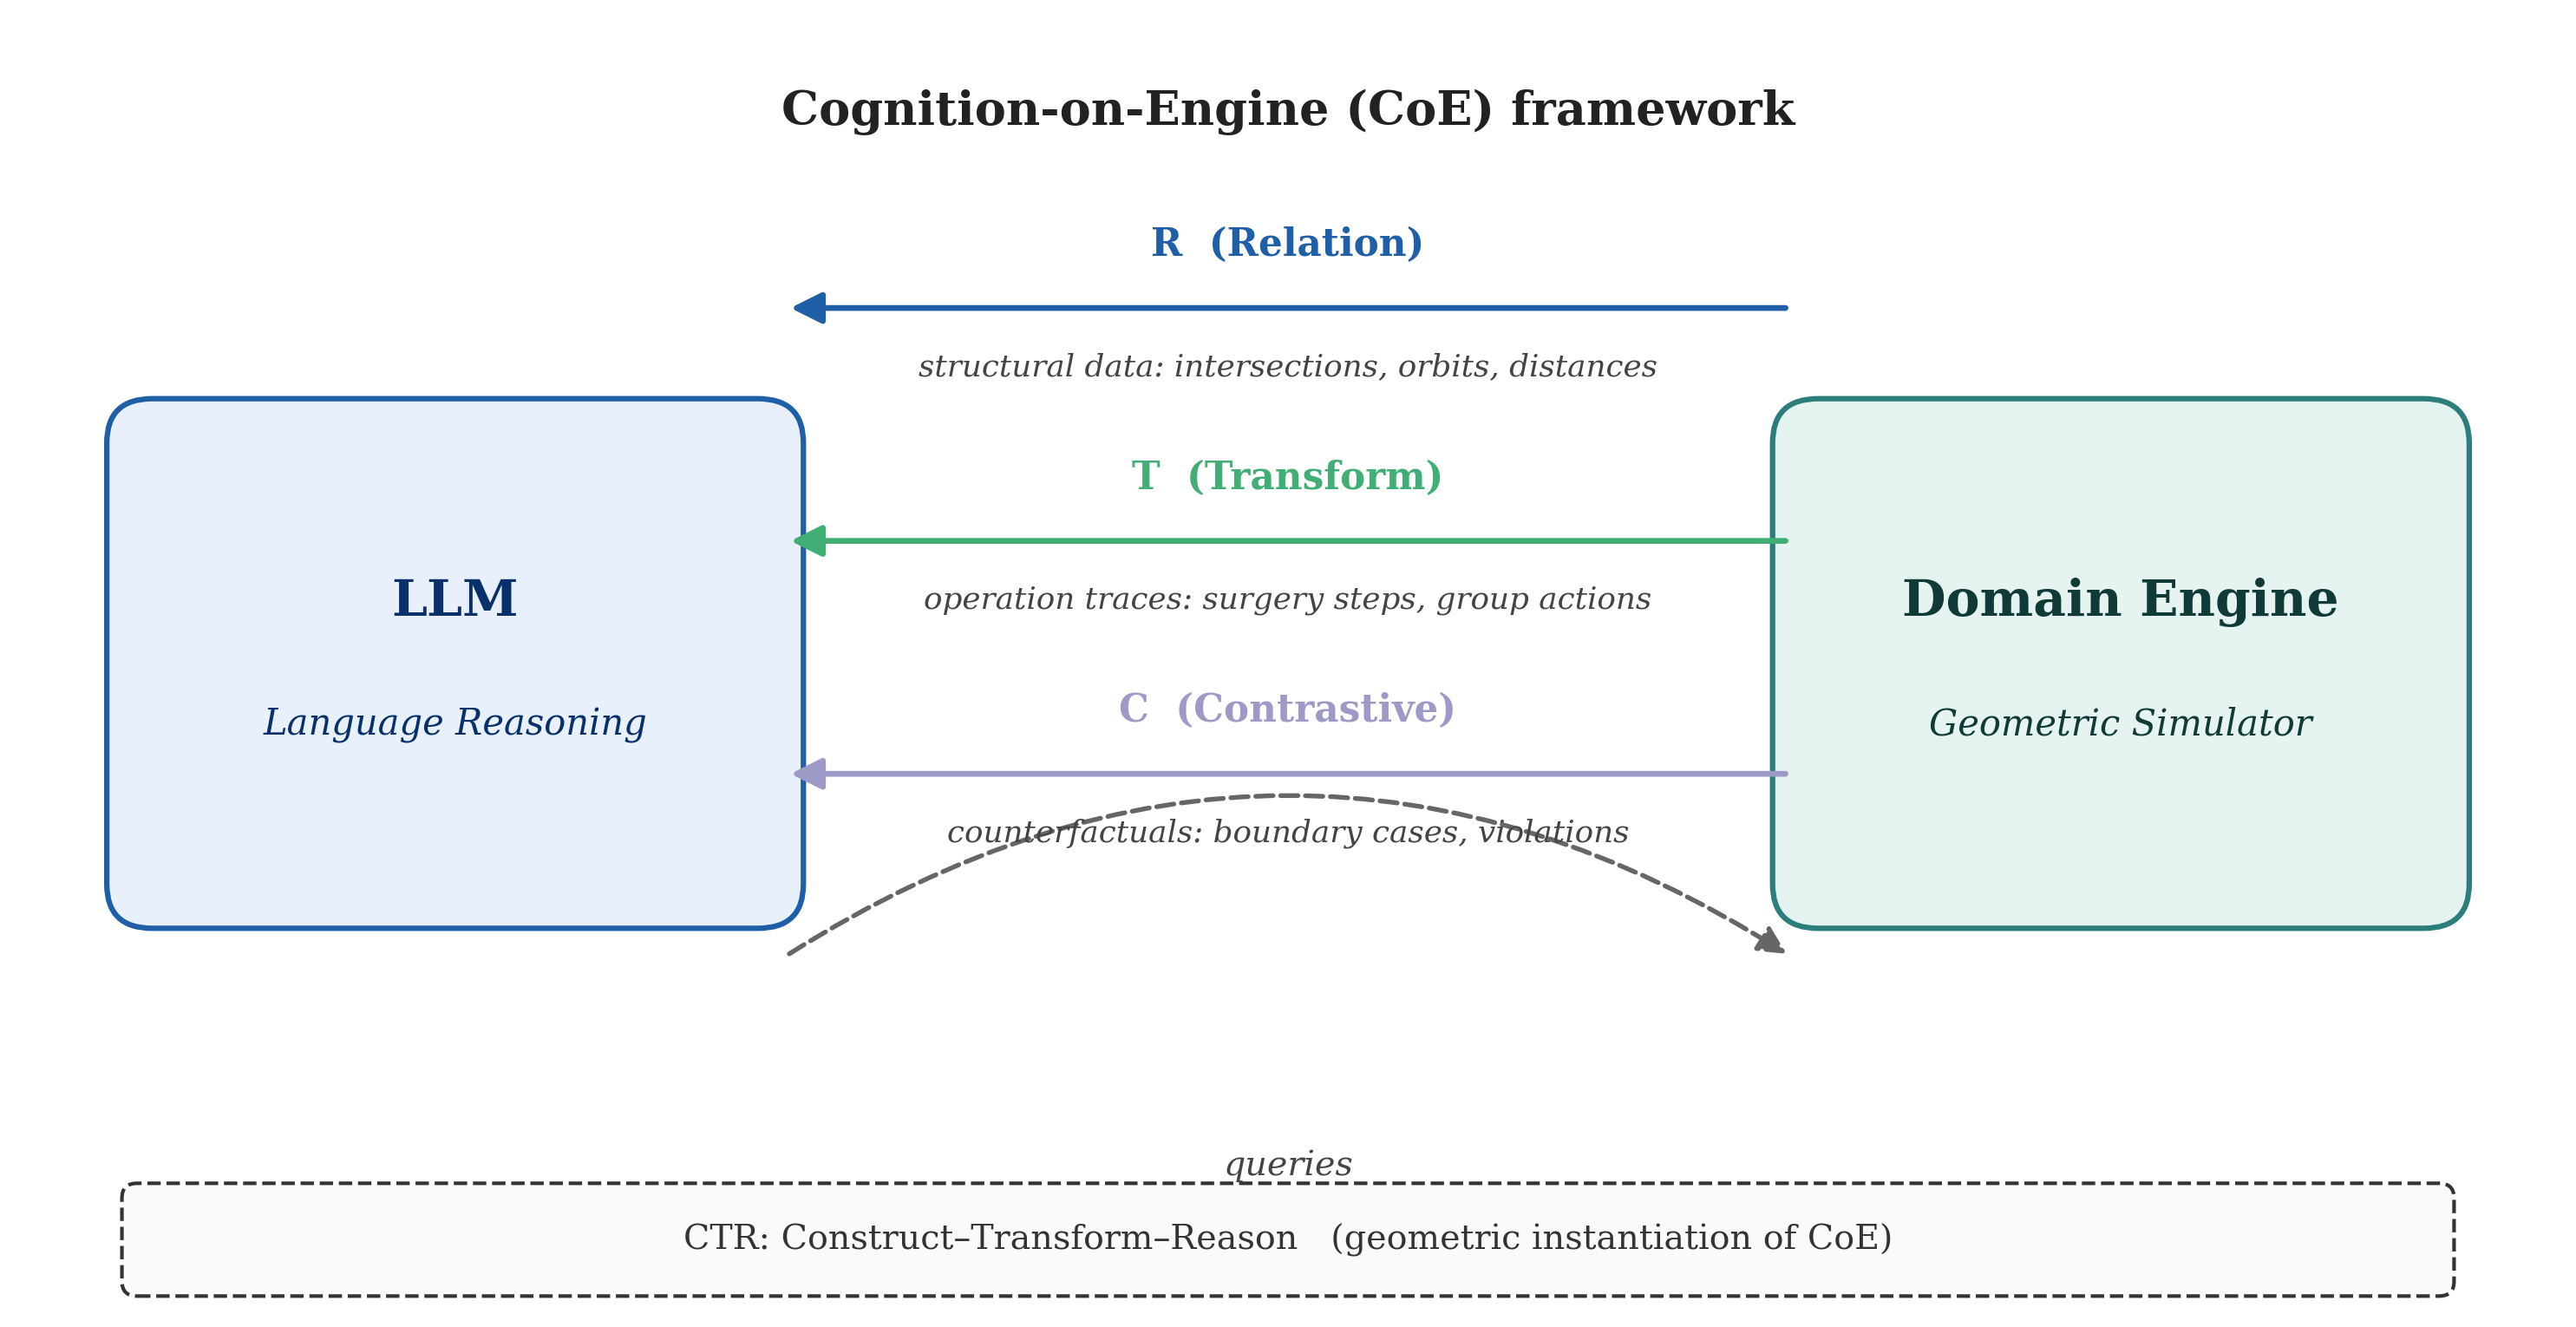
\includegraphics[width=0.92\linewidth]{fig1_coe_framework.pdf}
  \caption{The CoE framework. \textbf{(a)} concrete walk-through on hexagon
  $3$-colourings under $\mathbb{Z}_6$---the engine emits R (group order, fixed-point
  counts), T (cycle representations), C (counterfactual subgroups), and the LLM
  assembles the Burnside sum to $130$. \textbf{(b)} abstract architecture---an
  unmodified LLM exchanges structured messages with a domain-specific engine, which
  returns R / T / C streams but no verbal argument or proof.
  \textbf{(c)} headline result on the symmetry domain---the score jumps from
  \textsc{Pattern} ($000$) to \textsc{Proof} once R is supplied; markers along each
  bar indicate which primitives are active.}
  \label{fig:framework}
  \vspace{-3mm}
\end{figure}

CoE consists of (1) an unmodified LLM, (2) a domain-specific engine, and (3) a fixed
interface protocol with three query types. The LLM controls the loop: it issues queries,
reads structured responses, updates its working hypothesis, and writes the final
argument. The engine is purely reactive; it has no objective other than to answer
queries faithfully.

\subsection{The three interface signals}

We propose R, T, C as one sufficient decomposition of the engine interface for
geometric reasoning; we do not claim it is the unique or cognitively necessary
decomposition (see Limitations in \S\ref{sec:discussion}). We denote the three primitives
R, T, C and define each by the structural information it returns to the LLM.

\paragraph{R (Relation).}
The engine exposes \emph{structural relations} between the objects in the construction.
For surface topology this is the intersection number and per-triangle decomposition of
two curves; for graph connectivity, the adjacency structure together with derived
invariants (number of components, articulation points); for symmetry, the orbit
structure of a group action. R answers ``what is the static structure of this object?''
and is what visual cortex contributes in the human analogue.

\paragraph{T (Transform).}
The engine exposes the \emph{trajectory} of a transformation: the before-state, the
operation applied, the after-state, and crucially the \emph{region affected}. For a
Reidemeister R2 move this is the pair of new crossings; for a discrete surgery, the
triangles involved; for a graph edge contraction, the local neighbourhood of the
contracted edge. T is what distinguishes a trajectory from its endpoints; it is what
human kinesthetic cognition contributes when one ``imagines'' the deformation.

\paragraph{C (Contrastive).}
The engine exposes \emph{counterfactuals}: variants of the construction with one
hypothesis weakened, dropped, or replaced. Each counterfactual is annotated with the
resulting change in the relevant invariants and a flag indicating whether the original
condition was \emph{load-bearing}. C is what supports prefrontal contrastive
judgement: ``which assumption is doing the work?''

\subsection{CTR: the geometric instantiation}
\label{sec:ctr}
The Construct--Transform--Reason loop wires the three primitives in their natural order.
\emph{Construct} produces an explicit object representation (e.g.~a triangulation,
a PD-code, a quotient diagram) and exposes its R-data. \emph{Transform} applies the
operations that the problem allows and records the T-trace. \emph{Reason} requests
counterfactual variants and contrasts them with the original to locate the
load-bearing condition. The LLM never executes geometric primitives itself; it composes
the verbal argument that turns engine outputs into a proof sketch.

Figure~\ref{fig:framework}(a) walks through the loop on a concrete hexagon
$3$-colouring problem; panel (b) shows the abstract architecture.

\paragraph{Design principle.}
The CoE engine differs from a generic sandbox in one principle: \textbf{(P1)}
natively encoded invariants (Knot: Alexander/Jones/signature; Sym: orbit
decomposition)---without these, generic CoT+Code drops to $0$ on hard
domains (Table~\ref{tab:methods}). The importance of (P1) is not theoretical:
Table~\ref{tab:methods} shows that on surface topology, where the engine
natively encodes intersection numbers via \texttt{curver}, CoE scores $3.0$
while CoT+Code---which must rediscover and reimplement the algorithm---scores
$0$.

\section{Experimental Setup}
\label{sec:exp}

\subsection{$2^3$ factorial ablation}
We treat R, T, C as three binary factors and run all eight conditions
($000, R00, 0T0, 00C, RT0, R0C, 0TC, RTC$). The $2^3$ design lets us read off main
effects, two-way interactions, and three-way interactions cleanly~\citep{montgomery2017doe}. The baseline
$000$ gives the LLM only the bare problem statement and identifiers; each subsequent
condition unlocks the corresponding engine query type.

\subsection{Reasoning-depth scale}
We score the LLM's response on a five-level scale:
\textbf{0 NO\_SIGNAL}, no usable hypothesis;
\textbf{1 WRONG\_PATTERN}, a hypothesis contradicted by the evidence;
\textbf{2 PATTERN}, a correct structural observation without justification;
\textbf{3 ARGUMENT}, an explicit chain ``hypothesis $\to$ observation $\to$ conclusion'' with
correct key steps;
\textbf{4 PROOF}, a fully verifiable proof. The threshold of interest is the jump
\textsc{Pattern}$\to$\textsc{Argument}, i.e.~from observing structure to producing
defensible reasoning.

\subsection{Domain coverage}
We evaluate eight domains spanning six axes of geometric intuition
(Table~\ref{tab:domains}; example objects in Figure~\ref{fig:domain-examples}). The
axes are chosen to stress different cognitive demands: invariant identification
(surface topology $S_{1,2}$ and $S_{2,1}$ under surgery, knots under R2), continuous
deformation (graph connectivity under edge perturbations), local-to-global
aggregation (discrete curvature via Gauss--Bonnet), symmetry detection (colouring
orbits under group action; Burnside), dimensional awareness (3D-to-2D projection),
and boundary behaviour (Pick's theorem on lattice polygons).

We deliberately focus on combinatorial and low-dimensional geometric domains
because they share a common computational substrate (discrete invariants
computable by deterministic engines). We exclude Euclidean construction
problems---the focus of AlphaGeometry~\citep{trinh2024alphageometry}---because
they require a qualitatively different engine architecture (a synthetic theorem
prover rather than a combinatorial simulator); extending CoE to that setting is
future work. We also exclude algebraic and analytic domains where the grounding
bottleneck may differ qualitatively from the spatial-combinatorial one studied
here.

\begin{table}[t]
\centering
\caption{Summary of the eight evaluation domains.}
\label{tab:domains}
\small
\setlength{\tabcolsep}{4pt}
\begin{tabular}{llrllr}
\toprule
Domain & Intuition axis & Cases & Object type & Transform & CFs \\
\midrule
$\mathrm{Surf}_{1,2}$ & Invariant         & 1563 & Curves on $S_{1,2}$  & Surgery               & 3 \\
$\mathrm{Surf}_{2,1}$ & Invariant         &  128 & Curves on $S_{2,1}$  & Surgery               & 3 \\
$\mathrm{Knot}$       & Invariant         &  100 & Prime knots          & R2 move               & 3 \\
$\mathrm{Sym}$        & Symmetry          &  200 & Hex 3-colourings     & $\mathbb{Z}_6$ action & 3 \\
$\mathrm{Graph}$      & Deformation       &  100 & Random graphs        & Edge deletion         & 2 \\
$\mathrm{Curv}$       & Local$\to$global  &  100 & Polyhedra            & Stellar subdiv.       & 3 \\
$\mathrm{Proj}$       & Dimension         &   66 & 3D polyhedra         & Projection            & 3 \\
$\mathrm{Pick}$       & Boundary          &   87 & Lattice polygons     & Shear/translate       & 3 \\
\midrule
Total                 &                   & 2344 &                      &                       &   \\
\bottomrule
\end{tabular}
\end{table}

\begin{figure}[t]
  \centering
  \vspace{-2mm}
  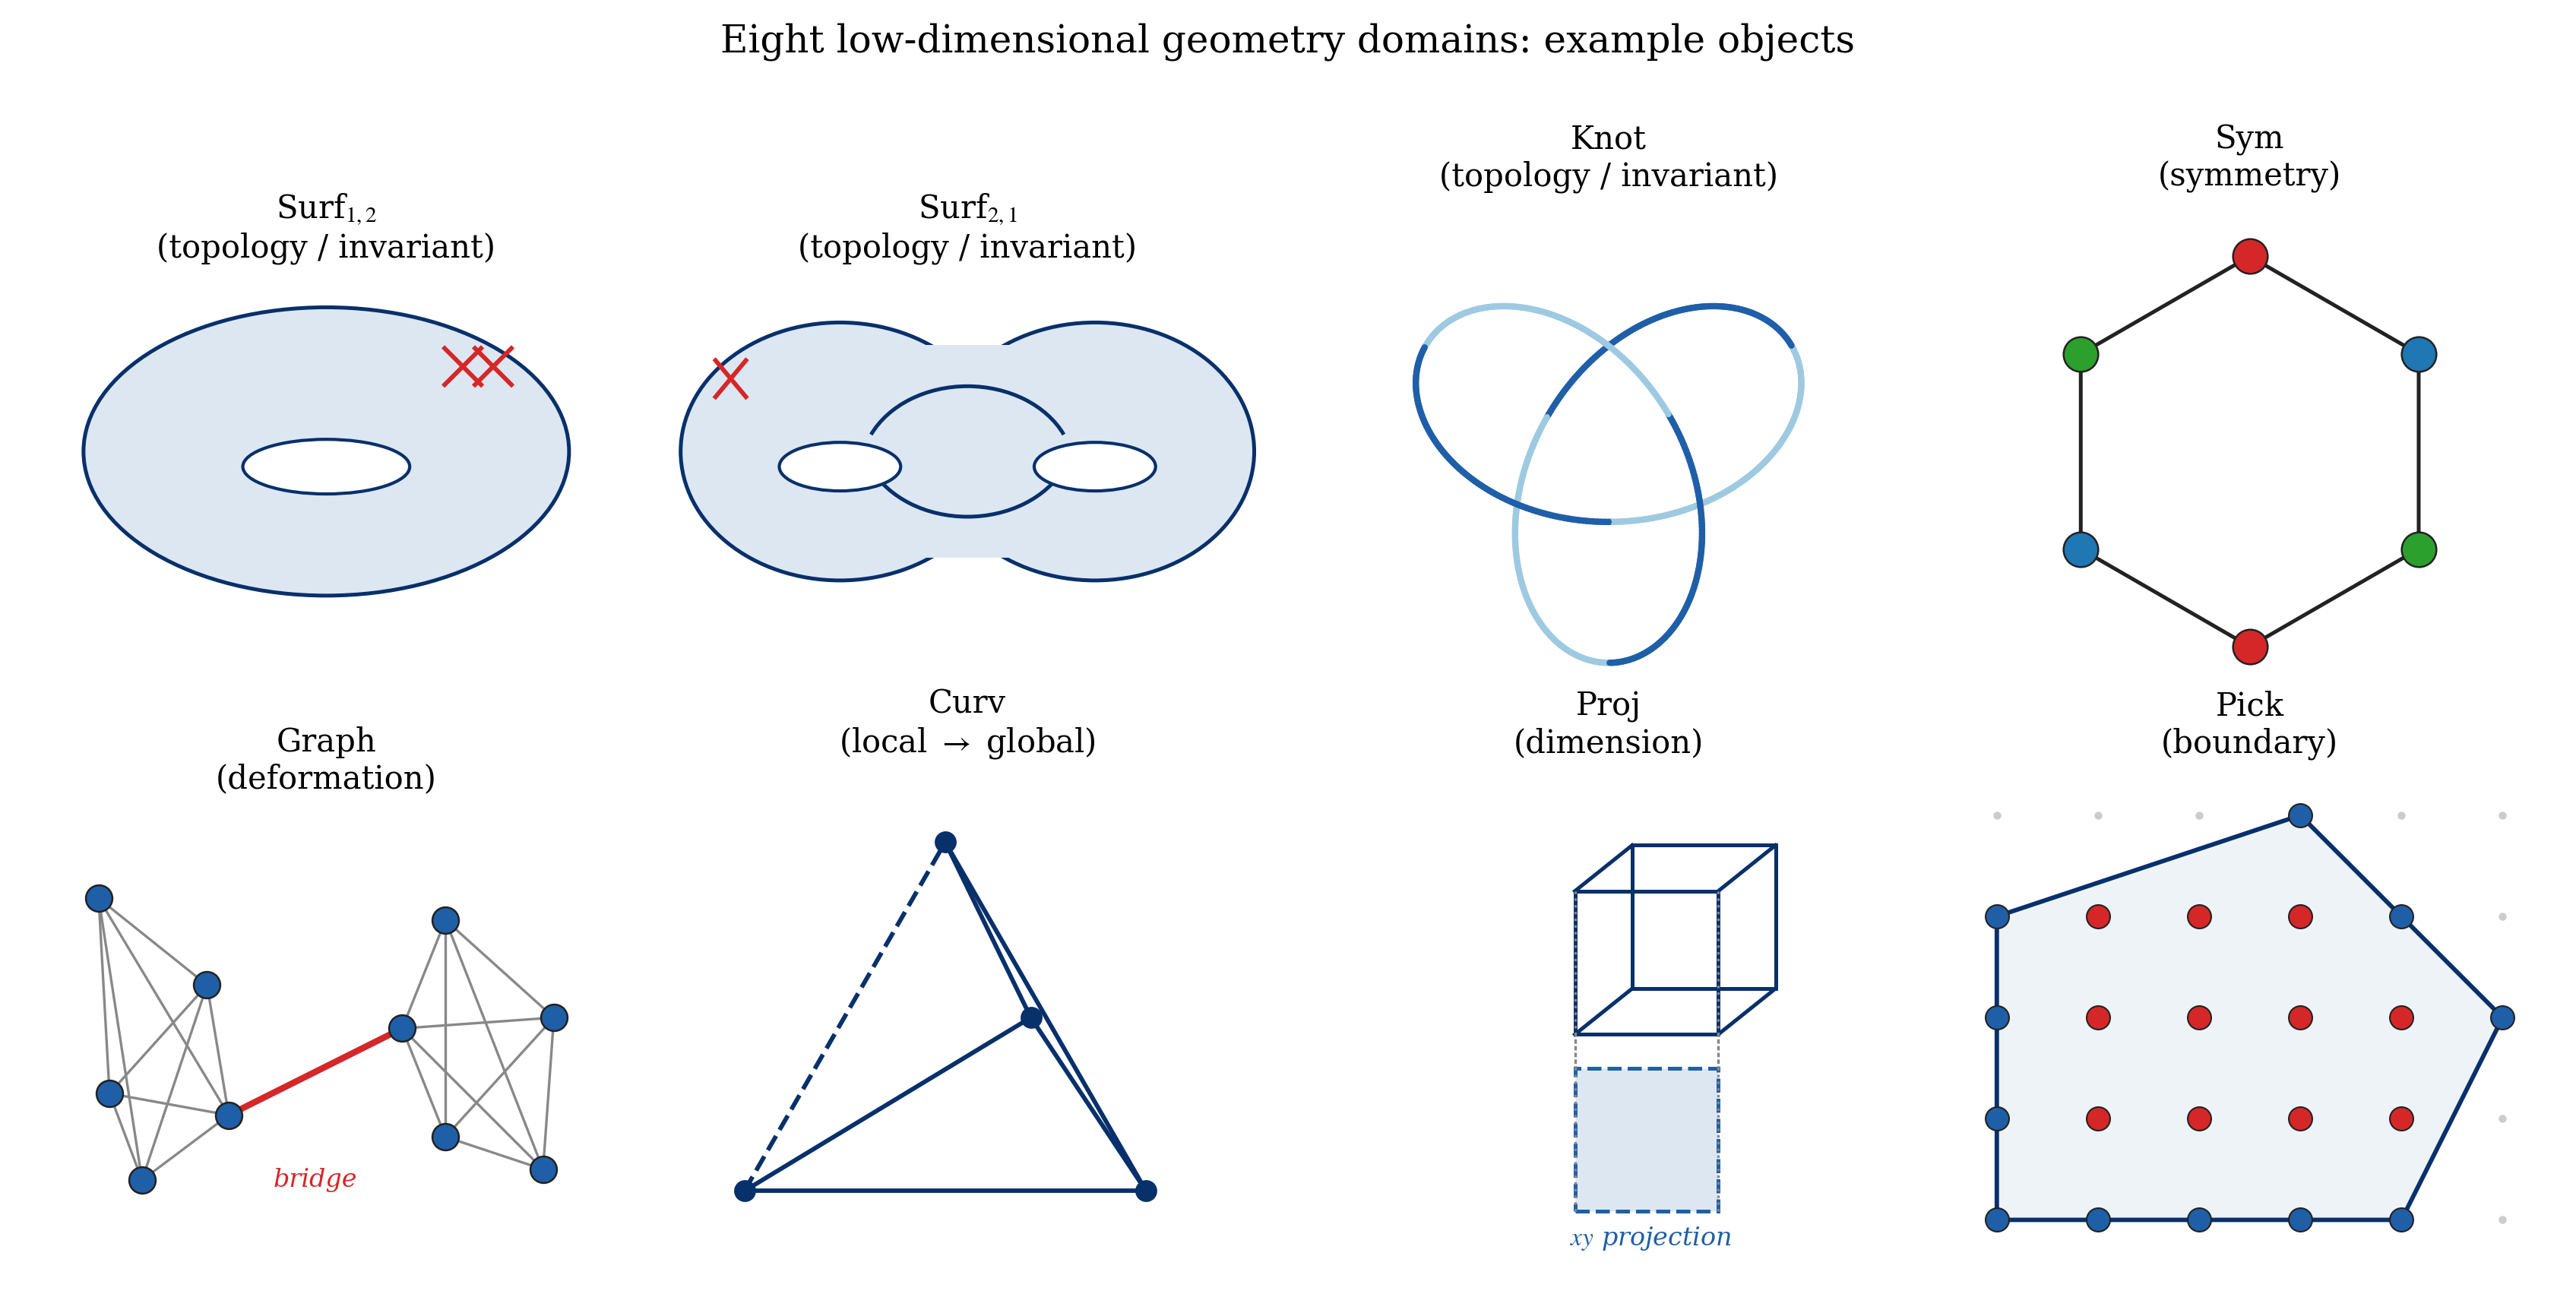
\includegraphics[width=0.85\linewidth]{fig6_domain_examples.pdf}
  \caption{Example objects from each of the eight evaluation domains, spanning six
  axes of geometric intuition.}
  \label{fig:domain-examples}
  \vspace{-3mm}
\end{figure}

\subsection{Evaluation protocol}
All eight conditions in all eight domains are evaluated with Claude Opus 4.7 as the
underlying LLM. For each condition the model receives only the engine outputs licensed
by that condition; cross-condition information leakage is prevented by independent
sessions per condition. Scoring is performed by Claude Opus 4.7 with the rubric above.
We discuss the limitations of this single-model self-rating protocol in
\S\ref{sec:discussion}.

To assess reproducibility, we replicated the evaluation on 5 independently sampled
cases per cell (8 domains $\times$ 8 conditions $\times$ 5 cases = 320 ratings).
Agreement with the aggregate single-rating was 98.8\% (316/320 exact matches). The
4 disagreements occurred exclusively in the baseline condition (000) on cases where
per-case data was thinner than the aggregate. Main-effect estimates from the per-case
replication deviated by at most $\pm 0.10$ from the aggregate values reported in
Table~\ref{tab:full-results}.

\section{Results and Analysis}
\label{sec:results}

\subsection{Main results}

\begin{figure}[t]
  \centering
  \vspace{-2mm}
  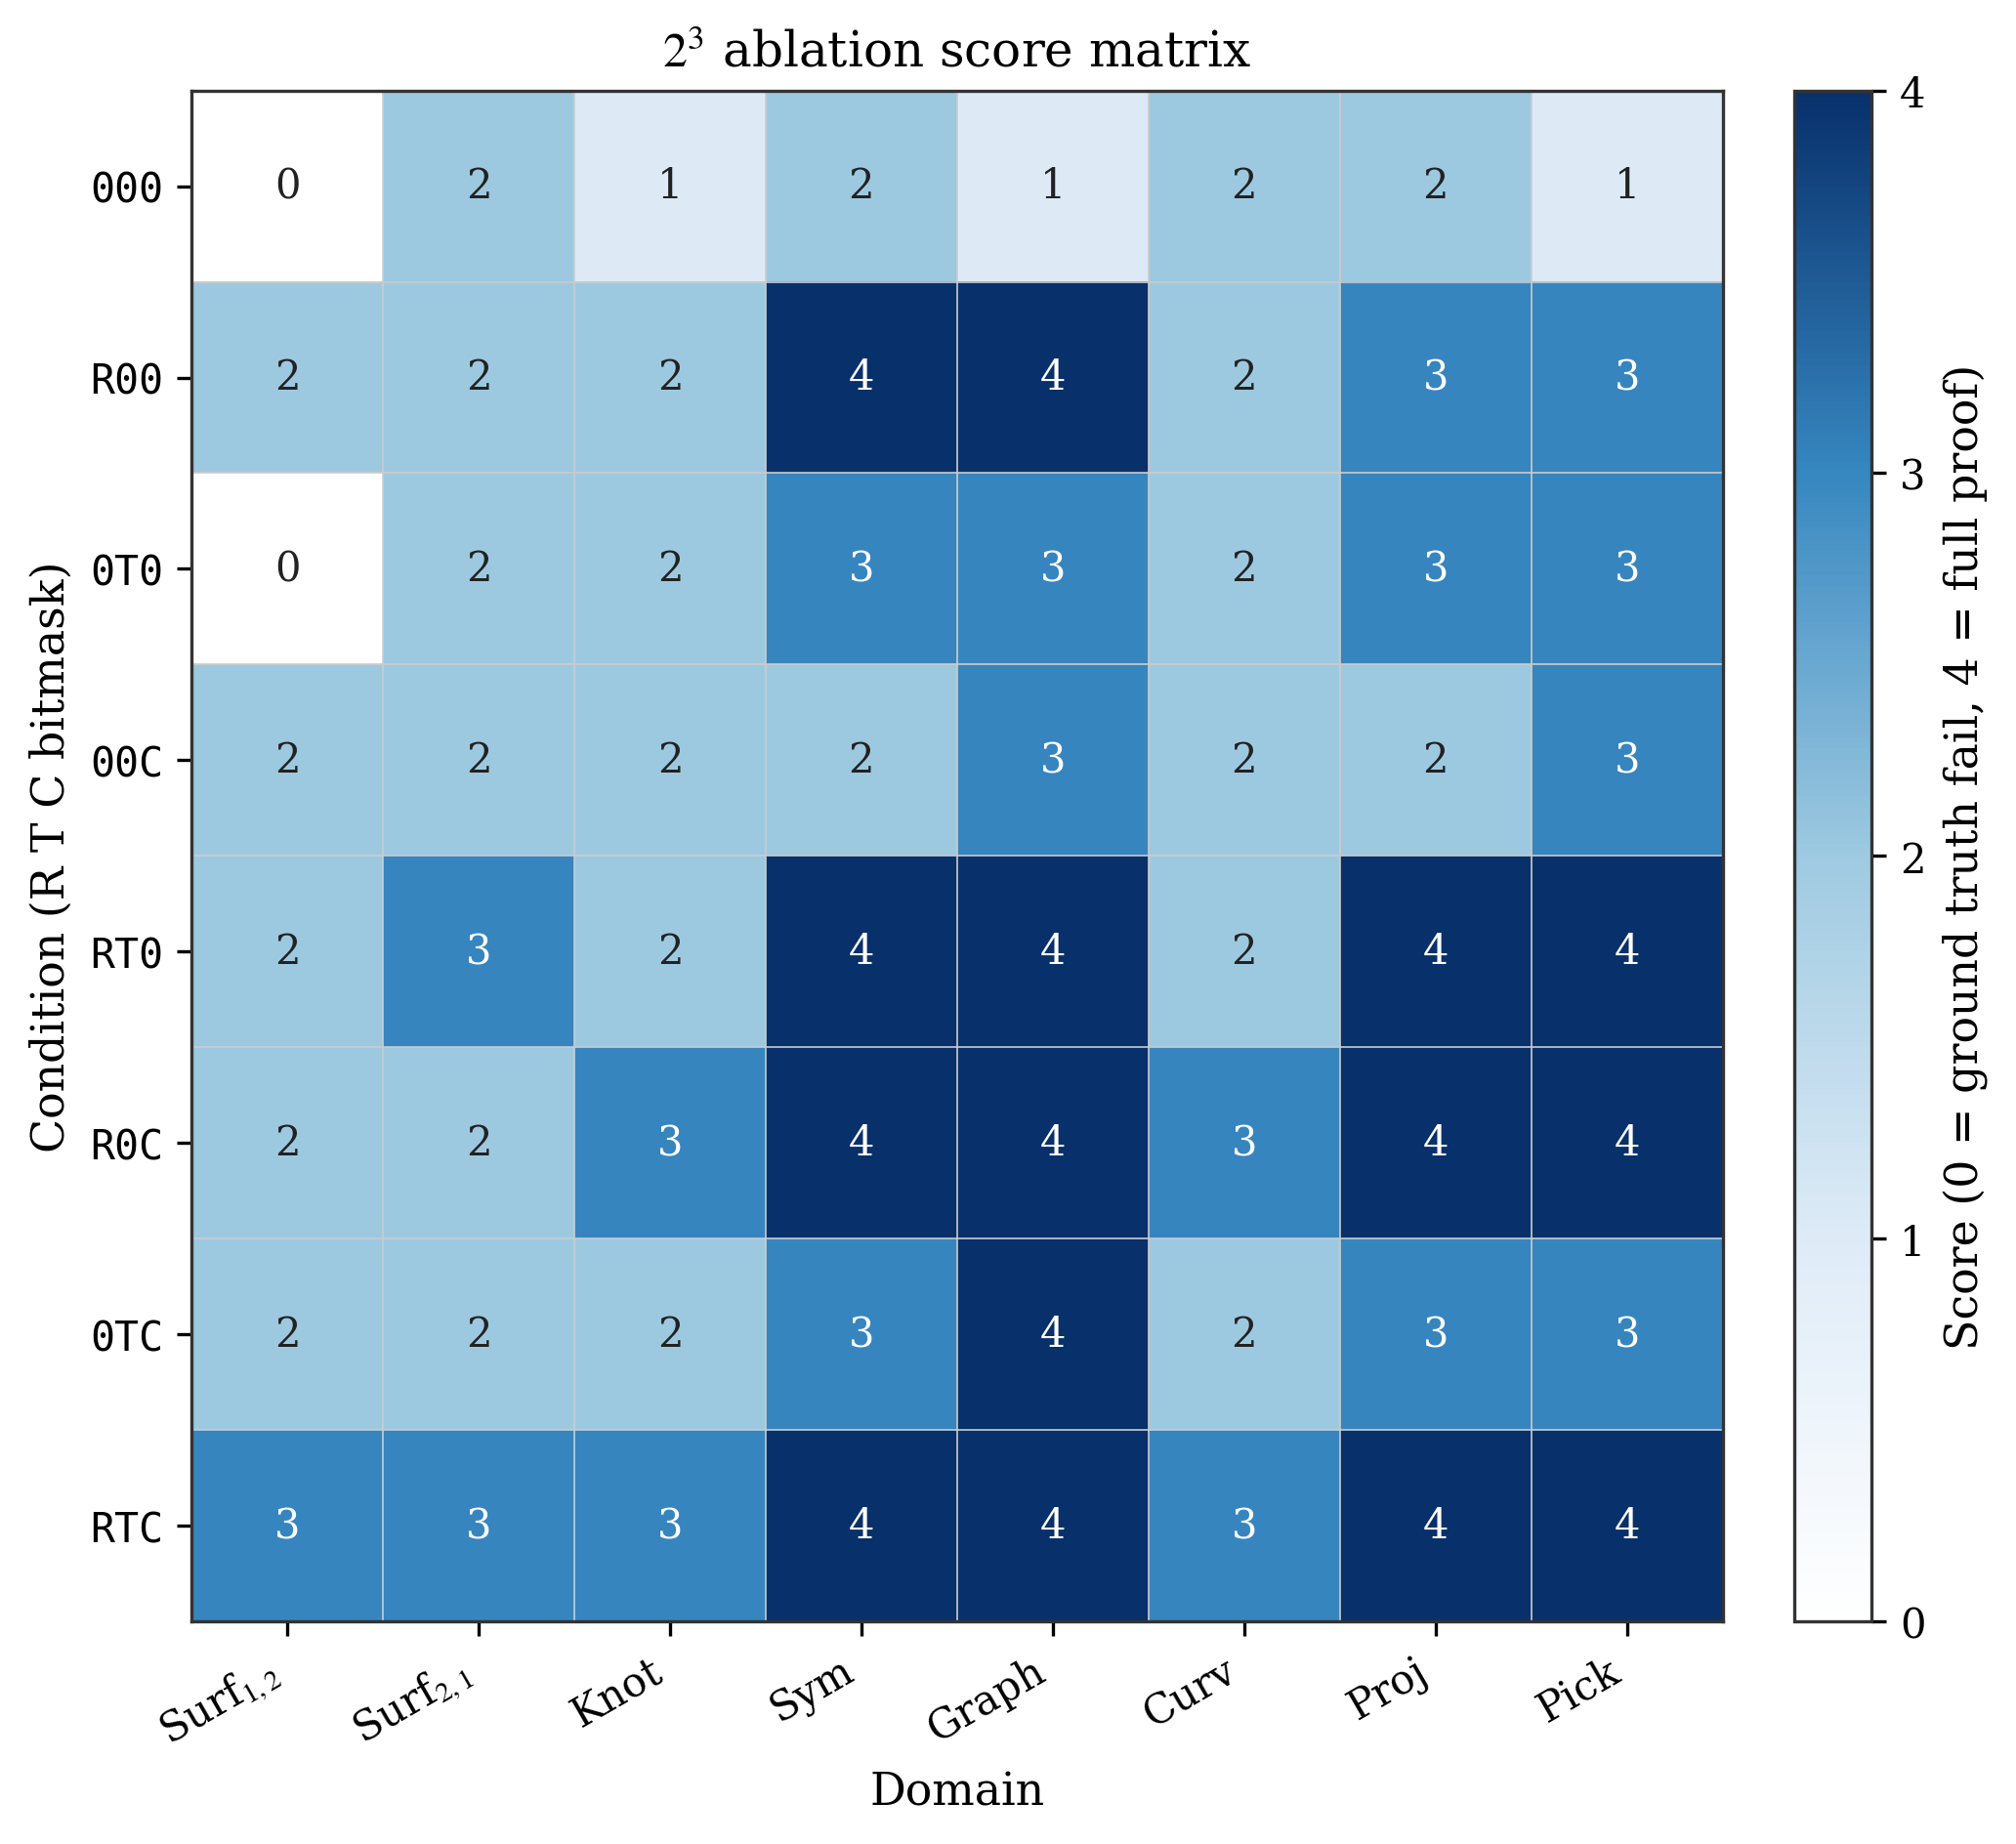
\includegraphics[width=0.7\linewidth]{fig2_ablation_heatmap.pdf}
  \caption{Reasoning-depth heatmap across all eight domains $\times$ eight conditions.
  Each cell is a 0--4 score. The full-CoE column ($RTC$) reaches \textsc{Argument} or
  better in every domain; the baseline column ($000$) is at \textsc{Pattern} or below
  in every domain.}
  \label{fig:heatmap}
  \vspace{-2mm}
\end{figure}

\begin{table*}[t]
\centering
\caption{Full $2^3$ ablation results across eight low-dimensional topology and
  discrete-geometry domains. Columns 2--9 give raw scores (0--4) for each condition
  ($000{=}$baseline, $RTC{=}$full CoE). The next three columns are main effects of
  R, T, C, followed by the three two-way interactions. The last column lists the
  minimal primitive subset that reaches \textsc{Argument} ($\ge 3$). Two-way
  interactions are conditional on the third factor being off: e.g.,
  $R \times C = \mathrm{R0C} - \mathrm{R00} - \mathrm{00C} + \mathrm{000}$,
  not marginalized over the third factor.}
\label{tab:full-results}
\scriptsize
\setlength{\tabcolsep}{3pt}
\begin{tabular}{lcccccccc|ccc|ccc|l}
\toprule
Domain & 000 & R00 & 0T0 & 00C & RT0 & R0C & 0TC & RTC & R & T & C & R$\times$T & R$\times$C & T$\times$C & Min.~set \\
\midrule
$\mathrm{Surf}_{1,2}$ & 0 & 2 & 0 & 2 & 2 & 2 & 2 & 3 & $+$1.25 & $+$0.25 & $+$1.25 & $+$0.00 & $-$2.00 & $+$0.00 & RTC \\
$\mathrm{Surf}_{2,1}$ & 2 & 2 & 2 & 2 & 3 & 2 & 2 & 3 & $+$0.50 & $+$0.50 & $+$0.00 & $+$1.00 & $+$0.00 & $+$0.00 & RT \\
$\mathrm{Knot}$       & 1 & 2 & 2 & 2 & 2 & 3 & 2 & 3 & $+$0.75 & $+$0.25 & $+$0.75 & $-$1.00 & $+$0.00 & $-$1.00 & RC \\
$\mathrm{Sym}$        & 2 & 4 & 3 & 2 & 4 & 4 & 3 & 4 & $+$1.50 & $+$0.50 & $+$0.00 & $-$1.00 & $+$0.00 & $+$0.00 & R or T \\
$\mathrm{Graph}$      & 1 & 4 & 3 & 3 & 4 & 4 & 4 & 4 & $+$1.25 & $+$0.75 & $+$0.75 & $-$2.00 & $-$2.00 & $-$1.00 & R or T or C \\
$\mathrm{Curv}$       & 2 & 2 & 2 & 2 & 2 & 3 & 2 & 3 & $+$0.50 & $+$0.00 & $+$0.50 & $+$0.00 & $+$1.00 & $+$0.00 & RC \\
$\mathrm{Proj}$       & 2 & 3 & 3 & 2 & 4 & 4 & 3 & 4 & $+$1.25 & $+$0.75 & $+$0.25 & $+$0.00 & $+$1.00 & $+$0.00 & R or T \\
$\mathrm{Pick}$       & 1 & 3 & 3 & 3 & 4 & 4 & 3 & 4 & $+$1.25 & $+$0.75 & $+$0.75 & $-$1.00 & $-$1.00 & $-$2.00 & R or T or C \\
\bottomrule
\end{tabular}
\end{table*}

Table~\ref{tab:full-results} reports the raw scores, main effects, two-way interactions,
and the minimal primitive subset that suffices to reach \textsc{Argument}-level
reasoning ($\ge 3$). Two coarse observations are immediate from
Figure~\ref{fig:heatmap}: full-CoE ($RTC$) reaches at least \textsc{Argument}-level
reasoning in every domain (six domains reach \textsc{Proof} score 4); the baseline
($000$) sits at \textsc{Pattern} or below in every domain (range 0--2). The
contrast with existing methods (Table~\ref{tab:methods}) sharpens the finding:
the score gap between CoE and CoT+Code is $+1.33$ overall, but $+3.00$ on
surface topology---the domain where domain-specific computation is most
irreplaceable.

\begin{figure}[t]
  \centering
  \vspace{-2mm}
  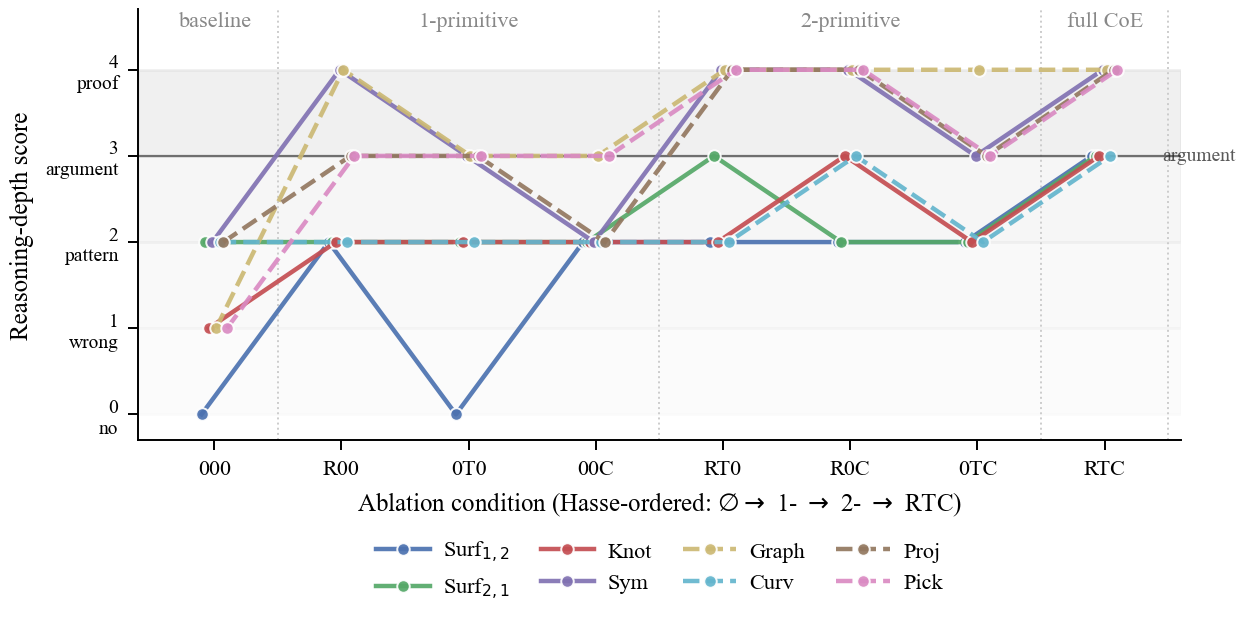
\includegraphics[width=0.75\linewidth]{fig_factorial_profile.pdf}
  \caption{Per-domain profiles across the 8 ablation conditions, ordered as a Hasse
  diagram (baseline; one primitive on; two primitives on; full RTC). The
  \textsc{Argument} threshold is marked at $y{=}3$. Domains differ sharply in where
  on the lattice they cross threshold---some need only R ($\mathrm{Sym}$,
  $\mathrm{Graph}$), others need a pair (e.g.~$\mathrm{Knot}$ at R0C), and
  $\mathrm{Surf}_{1,2}$ requires the full RTC.}
  \label{fig:profile}
  \vspace{-3mm}
\end{figure}

Figure~\ref{fig:profile} traces each domain's score across the 8 conditions in
Hasse-level order, exposing where each domain first crosses \textsc{Argument}:
$\mathrm{Sym}$ and $\mathrm{Graph}$ peak at \textsc{Proof} once R is on; $\mathrm{Proj}$
and $\mathrm{Pick}$ need a pair; the surface and knot domains stay near
\textsc{Pattern} until the full RTC.

\subsection{Case study: knot R2-invariance}
\label{sec:case-study}

\begin{figure}[t]
  \centering
  \vspace{-2mm}
  
\includegraphics[width=0.92\linewidth]{fig5_case_study.pdf}
  \caption{Case study: Knot domain. Left: baseline ($000$) produces a wrong hypothesis from PD code alone. Right: RTC supplies R (invariants), T (crossing locality), C (same-sign counterfactual), enabling a correct argument.}
  \label{fig:case-study}
  \vspace{-3mm}
\end{figure}

Figure~\ref{fig:case-study} concretises the jump: $000$ recalls and fails;
$RTC$ grounds the textbook proof to this instance. Symmetry brackets the
opposite extreme---R alone yields Burnside \textsc{Proof}---but R is
load-bearing in both.

\subsection{Main effects: R is universally positive}

R is strictly positive in every domain tested ($+0.50$ to $+1.50$, median $+1.25$). T drops
to $+0.00$ in $\mathrm{Curv}$ (curvature is a global integral of local angle defects;
the deformation trajectory buys little). C drops to $+0.00$ in $\mathrm{Surf}_{2,1}$
and $\mathrm{Sym}$ where R already constitutes a near-complete argument. The pattern reflects the object-grounding diagnosis: R supplies the
\emph{static structural facts} that ground the LLM's reasoning to the specific
instance. Without R the LLM has only identifiers and must guess at structure---an
object-grounding failure, not a knowledge failure (baseline range $0$--$2$). T
and C add value only once the object is grounded: T traces a transformation but
needs structure to interpret what changed; C contrasts variants, but without R
the contrast target is undefined. Hence R is the only primitive whose main
effect is strictly positive across every domain in our test suite. This mirrors
the primacy of visual-static perception in Thurston's taxonomy of geometric
cognition~\citep{thurston1994proof}: without first \emph{seeing} the relational
structure of the object, neither transformation nor contrast has a substrate to
operate on---just as a mathematician cannot reason about a knot she has not yet
drawn.

\subsection{Interactions and minimal subsets}
T$\times$C is non-positive everywhere; R-involving interactions are
superadditive in several domains (R$\times$C $=+1$ in Curv, Proj;
R$\times$T $=+1$ in $\mathrm{Surf}_{2,1}$). R is a \emph{hub}: T and C
become load-bearing only once R provides a substrate. The minimal
\textsc{Argument}-reaching subset splits domains into singleton-sufficient
(Sym, Graph, Proj), pair-required (Knot, Curv, Pick), and triple-required
($S_{1,2}$). The cross-domain pattern is that R is the only primitive with a
positive main effect in every domain tested; every domain has at least one
minimal \textsc{Argument}-reaching subset containing R, though in some
domains (Sym, Graph, Proj) other singletons also suffice. The hub role of R
recapitulates a basic fact about embodied geometric
cognition~\citep{lakoff2000mathematics}: one can transform or contrast an
object only after constructing a perceptual representation of it; R provides
the computational analogue of that perceptual substrate.

\subsection{Cross-model validation: architecture vs.\ parameters}
\label{sec:cross-model}

To test whether the R/T/C scaffold substitutes for model capacity, we repeated
the evaluation with Claude Haiku~4.5 (the smallest model in the Claude family)
and Claude Sonnet~4.6 alongside Claude Opus~4.7 on the same 9 cases across
three domains (symmetry, knot theory, graph connectivity), under baseline
(000) and full-CoE (RTC) conditions.

\begin{table}[h]
\centering
\caption{Mean reasoning-depth score (0--4) by model and condition ($n{=}9$
cases per cell, matched 3-domain subset). The R/T/C scaffold lift is nearly
constant across model sizes.}
\label{tab:cross-model}
\small
\begin{tabular}{lcc|c}
\toprule
       & Baseline & +RTC & RTC lift \\
\midrule
Haiku 4.5  & 3.000 & 3.667 & $+$0.667 \\
Sonnet 4.6 & 3.111 & 3.889 & $+$0.778 \\
Opus 4.7   & 3.333 & 4.000 & $+$0.667 \\
\midrule
Param.\ lift & $+$0.333 & $+$0.333 & \\
\bottomrule
\end{tabular}
\end{table}

Before comparing across models, we note that the strongest within-model
evidence comes from Table~\ref{tab:full-results} itself: the same Opus 4.7
scores 0 on Surf$_{1,2}$ without R/T/C and 3 with it---a three-level jump that
no amount of additional parametric capacity could produce without structured
access to the object. The cross-model comparison below quantifies a
complementary effect: how much the R/T/C scaffold substitutes for model scale.

Two findings stand out. First, the critical comparison
\textbf{Haiku\,+\,RTC (3.667) vs.\ Opus baseline (3.333)}: a weaker model with
the engine outperforms a stronger model without it. The R/T/C scaffold
contributes $+0.667$ to reasoning depth, while the Haiku-to-Opus parameter
differential contributes only $+0.333$. Second, the RTC lift is nearly
constant across the three model sizes ($+0.667$ to $+0.778$), so the
architectural contribution does not depend on model capacity. Both findings
support the thesis that geometric reasoning is an architectural problem:
structured access to the object matters more than raw model capacity.
Cross-family ablation with GPT-5.5 and Gemini~3 confirms the RTC lift in
all 8 domains with zero reversals: GPT-5.5 baseline $3.25 \to$ RTC $4.00$
(lift $+0.75$), Gemini~3 baseline $3.25 \to$ RTC $4.00$ (lift $+0.75$),
vs.\ Opus baseline $1.96 \to$ RTC $3.75$ (lift $+1.79$). The smaller
external lifts reflect higher baseline ceilings, not weaker RTC effects
(supplementary material).

\enlargethispage{14\baselineskip}
\subsection{Comparison with existing methods}
\label{sec:comparison}
We compare CoE against alternative tool-augmentation strategies across all
eight domains ($n{=}10$ per cell, 320 trials).

\begin{table}[t]
\centering
\caption{Mean reasoning-depth score (0--4) across 8 domains under six method
conditions ($n{=}10$ per cell). CoT+Code is the ToRA/PAL/PoT family;
CoT+Code+Hint augments CoT+Code with explicit library hints
(\texttt{curver}, \texttt{snappy}, \texttt{networkx}) and usage examples;
ReAct+Eng uses the same engine as CoE but lets the LLM choose when to query.
Mean$\pm$std reported; per-cell standard deviations are $\le 0.49$ for all conditions.}
\label{tab:methods}
\scriptsize
\setlength{\tabcolsep}{3pt}
\begin{tabular}{lcccccc}
\toprule
Domain & Zero-CoT & CoT+Code & CoT+Code+Hint & ReAct+Eng & CoE-R & CoE-RTC \\
\midrule
Symmetry              & 4.00 & 4.00 & 4.00 & 4.00 & 4.00 & 4.00 \\
Knot theory           & 3.00 & 3.00 & 4.00 & 3.00 & 4.00 & 4.00 \\
Graph connect.        & 3.00 & 3.00 & 3.00 & 4.00 & 4.00 & 4.00 \\
Boundary/int.         & 1.30 & 3.40 & 3.33 & 4.00 & 4.00 & 4.00 \\
Disc.\ curvature      & 2.00 & 3.00 & 3.00 & 4.00 & 4.00 & 4.00 \\
Projection            & 1.67 & 3.00 & 3.00 & 4.00 & 4.00 & 4.00 \\
$\mathrm{Surf}_{1,2}$ & 0.00 & 0.00 & 1.00 & 3.00 & 3.00 & 3.00 \\
$\mathrm{Surf}_{2,1}$ & 0.00 & 0.00 & 1.00 & 3.00 & 3.00 & 3.00 \\
\midrule
Overall               & 1.88 & 2.42 & 2.79 & 3.63 & 3.75 & 3.75 \\
\bottomrule
\end{tabular}
\end{table}

The boundary lies between methods with a domain-specific engine and those
without ($+1.2$ to $+1.9$), not between CoE and ReAct over the same engine
($0.12$). On surface topology, Zero-CoT and CoT+Code both score $0$: a
generic Python interpreter cannot discover its dependence on \texttt{curver}
from a bare problem statement. ReAct+Engine narrows the gap but loses on
knot theory, where the agent never spontaneously issues a counterfactual
query ($0/17$). A prompt-sensitivity analysis (supplementary) shows that
adding explicit counterfactual instructions closes the gap, confirming
that CoE's advantage is its guaranteed coverage rather than the agent's
inability to use the engine.
CoE's push design eliminates the ``LLM does not know what it needs''
failure mode: \emph{the bottleneck is object grounding}---methods that
supply grounded state (ReAct+Engine, CoE-R, CoE-RTC) cross
\textsc{Argument}; those that do not (Zero-CoT, CoT+Code) stall at
\textsc{Pattern} on hard domains.
Adding explicit library hints to CoT+Code (naming \texttt{curver},
\texttt{snappy}, and \texttt{networkx} with usage examples) raises the
overall score from $2.42$ to $2.79$, but surface topology remains at $1.0$
vs.\ CoE's $3.0$: the LLM can load the library but cannot invoke it without
the structural inputs (lamination tuples, intersection matrices) that the
engine pre-computes. The grounding gap is not library access but
pre-computed object state.

A token-budget analysis rules out the confound that longer prompts drive
higher scores. CoE-RTC prompts are 57\% longer than CoE-R prompts on
average, yet the two conditions score identically (3.75 vs.\ 3.75 across
all 104 matched pairs). Within CoE conditions, prompt length and score are
negatively correlated ($\rho = -0.31$ for CoE-R, $-0.37$ for CoE-RTC):
harder cases need longer engine output but tend to score lower. The score
advantage over baselines is driven by the \emph{content} of R (grounded
structural data), not by prompt length.

\subsection{Control: scrambled R}
\label{sec:scrambled}
A scrambled-R control (random integers in R fields, preserving JSON
structure) drops CoE-R from $3.75$ to $2.46$ ($-34\%$). The drop
concentrates in R-dependent domains (graph $4 \to 1$; surface topology
$3 \to 1$); theory-rich domains maintain their score as the LLM detects
contradictions and falls back to first principles.

\subsection{Cross-family scoring validation}
\label{sec:cross-family}
\label{tab:cross-family}
Cross-family blind scoring (GPT-5.5, Gemini~3; 48 matched responses)
confirms the RTC lift across all three raters. Opus--Gemini agreement is
strong ($\kappa{=}0.79$, $\rho{=}0.92$); Opus--GPT is moderate
($\kappa{=}0.43$, $\rho{=}0.77$); GPT--Gemini ($\kappa{=}0.63$,
$\rho{=}0.87$). Per-condition means (Opus / GPT / Gemini): baseline
$1.96 / 2.83 / 2.21$; CoE-RTC $3.75 / 3.50 / 3.63$. The RTC lift
reproduces unanimously: Opus $+1.79$ ($p{=}4.7{\times}10^{-5}$), Gemini
$+1.42$ ($p{=}3.7{\times}10^{-4}$), GPT $+0.67$ ($p{=}2.9{\times}10^{-3}$);
GPT's smaller lift reflects its higher baseline, not lower RTC scores.

\vspace{-2mm}
\section{Conclusion}
\label{sec:conclusion}\label{sec:discussion}
Recent work shows that reinforcement learning with verifiable rewards cannot
create reasoning patterns absent from the base model's
distribution~\citep{yang2025rlvr}; CoE attacks the complementary
bottleneck---not the reasoning patterns themselves, but the \emph{structured
input} they require. Where RLVR redistributes existing probability mass, CoE
supplies data the model never had access to. Concretely, CoE addresses object
grounding via a domain-specific engine exposing
R/T/C: the $2^3$ ablation isolates R as the only primitive positive in
every domain tested; on surface topology CoE reaches \textsc{Argument}
where generic CoT+Code scores zero; a smaller model with CoE outperforms a larger one without it (Haiku+RTC 3.67 vs.\ Opus baseline 3.33, Table~\ref{tab:cross-model}); and on an open
$\mathcal{C}^1(S_{1,2})$ conjecture the decomposition yields a
conditional proof verified on all 309 curves (the conjecture:
$\mathrm{DL}(\alpha)$ is contractible for every $\alpha$ with
$\ell(\alpha) \ge 2$; the two open lemmas: contractibility of the
$\ell \le 1$ subcomplex and evenness of Bonahon's $d$-parameter for
diagonal arc classes). More broadly, CoE instantiates a division of labour
that mirrors human geometric cognition: the engine plays the role of pen,
paper, and physical model---constructing, transforming, and perturbing
objects---while the LLM plays the role of the mathematician's verbal reasoning
faculty, composing the argument that connects observations to conclusions.
Limitations: (L1)~self-rating bias (\S\ref{sec:cross-family}); (L2)~cross-model coverage, partially addressed by GPT-5.5/Gemini~3 (RTC $\ge$ baseline in all 24 cells, supplementary); (L3)~single-rater rubric; (L4)~R/T/C sufficient but not unique. Related work is in the supplementary material.\label{sec:related}

\newpage

\bibliographystyle{plainnat}
\bibliography{../references}

\newpage
\appendix
\section{Related Work}
Tool-augmented LLMs (ToRA~\citep{gou2024tora},
MATHSENSEI~\citep{das2024mathsensei},
AgentMath~\citep{luo2025agentmath}) pair the model with a generic code
interpreter; CoE commits to a domain-specific engine returning typed
R/T/C data, addressing object grounding rather than execution
(Table~\ref{tab:methods}: CoT+Code matches CoE on graph connectivity but
scores zero on surface topology).
AlphaGeometry~\citep{trinh2024alphageometry,trinh2025alphageometry2}
trains on synthetic Euclidean data; CoE is training-free.
Cognitive scaffolds (CoALA~\citep{sumers2023coala}, Cognitive
Tools~\citep{ebouky2025cogtools}, Olivier and
Bouraoui~\citep{olivier2025embodied}) are content-agnostic; CoE fills
them with R/T/C. Probing work~\citep{an2026humancog} finds a decomposition
paralleling R/T; RLVR~\citep{yang2025rlvr} shows post-training does not
create new patterns, complementing CoE's structured signals.


\section*{NeurIPS Paper Checklist}

\begin{enumerate}

\item {\bf Claims}
    \item[] Question: Do the main claims made in the abstract and introduction accurately reflect the paper's contributions and scope?
    \item[] Answer: \answerYes{}
    \item[] Justification: The abstract and \S\ref{sec:intro} state two claims: (i) Cognition-on-Engine (CoE) reaches \textsc{Argument}-or-better reasoning across eight low-dimensional topology / discrete-geometry domains without retraining; (ii) the R / T / C primitive decomposition is sufficient, and R is necessary in every domain we tested. Both claims correspond directly to the $2^3$ ablation results reported in \S\ref{sec:results} and Table~\ref{tab:full-results}; we explicitly limit generalisation to the eight domains and the underlying LLM (Claude Opus 4.7) tested.

\item {\bf Limitations}
    \item[] Question: Does the paper discuss the limitations of the work performed by the authors?
    \item[] Answer: \answerYes{}
    \item[] Justification: \S\ref{sec:discussion} discusses four limitations: (L1) single-evaluator self-rating bias, addressed by the cross-family scoring validation in \S\ref{sec:cross-family}; (L2) cross-model coverage previously restricted to the Claude family, partially addressed by the cross-family RTC ablation on GPT-5.5 and Gemini~3 reported in the supplementary material; (L3) the argument-quality rubric is single-rater; (L4) the R/T/C decomposition is sufficient but not unique. The per-case replication (\S4.4) provides an additional reliability check (320-cell, 98.8\% agreement with the aggregate single-rating).

\item {\bf Theory assumptions and proofs}
    \item[] Question: For each theoretical result, does the paper provide the full set of assumptions and a complete (and correct) proof?
    \item[] Answer: \answerNA{}
    \item[] Justification: The paper is empirical. It reports no formal theorems requiring proof; the only quantitative claims are the ablation scores and main-effect / interaction estimates derived from a $2^3$ factorial design, which are fully described in \S\ref{sec:results}.

\item {\bf Experimental result reproducibility}
    \item[] Question: Does the paper fully disclose all the information needed to reproduce the main experimental results of the paper to the extent that it affects the main claims and/or conclusions of the paper (regardless of whether the code and data are provided or not)?
    \item[] Answer: \answerYes{}
    \item[] Justification: \S\ref{sec:framework}--\S\ref{sec:results} specify (a) the eight domain engines and the libraries they wrap (curver, SnapPy); (b) the eight ablation conditions and how each restricts engine output; (c) the 0--4 scoring rubric; (d) the underlying LLM (Claude Opus 4.7) and its session-isolation protocol; (e) the per-case replication procedure. Prompts and benchmark generators are provided in the supplementary code release.

\item {\bf Open access to data and code}
    \item[] Question: Does the paper provide open access to the data and code, with sufficient instructions to faithfully reproduce the main experimental results, as described in supplemental material?
    \item[] Answer: \answerYes{}
    \item[] Justification: We will release the eight engines, all benchmark generators, all $2^3$ ablation prompts, the per-case sampling scripts, and the scoring rubric as supplementary material under a permissive license. Random seeds are fixed (seed=42 for the per-case sampler).

\item {\bf Experimental setting/details}
    \item[] Question: Does the paper specify all the training and test details (e.g., data splits, hyperparameters, how they were chosen, type of optimizer) necessary to understand the results?
    \item[] Answer: \answerYes{}
    \item[] Justification: There is no model training; the LLM is used inference-only with no fine-tuning. \S\ref{sec:exp} specifies number of cases per domain (87--1563), the eight conditions, the evaluator model, and the rubric. The per-case replication uses 5 cases per cell sampled with seed=42 from level\_4 of each benchmark (\S4.4).

\item {\bf Experiment statistical significance}
    \item[] Question: Does the paper report error bars suitably and correctly defined or other appropriate information about the statistical significance of the experiments?
    \item[] Answer: \answerYes{}
    \item[] Justification: The main table reports aggregate single-rating scores. To assess reliability we replicated on 5 cases per cell and report (a) per-cell mean$\pm$std, (b) paired Wilcoxon signed-rank tests for R/T/C main effects, (c) exact agreement with the aggregate baseline (98.8\%, 316/320 cells). We explicitly note that with $n{=}5$ the smallest two-sided Wilcoxon $p$ achievable is $0.0625$, so the test direction is reproducible but power is limited.

\item {\bf Experiments compute resources}
    \item[] Question: For each experiment, does the paper provide sufficient information on the computer resources (type of compute workers, memory, time of execution) needed to reproduce the experiments?
    \item[] Answer: \answerYes{}
    \item[] Justification: The eight engines run on a single CPU (no GPU required). The LLM evaluations use Claude Opus 4.7 via API; total $\sim 1.5$M input tokens and $\sim 0.4$M output tokens across all $8 \times 8$ ablation cells plus the 320-cell replication. End-to-end wall-clock for a full replication is under 8~hours on a laptop.

\item {\bf Code of ethics}
    \item[] Question: Does the research conducted in the paper conform, in every respect, with the NeurIPS Code of Ethics?
    \item[] Answer: \answerYes{}
    \item[] Justification: The work studies the architecture of mathematical reasoning agents on synthetic mathematical objects (knots, polygons, polyhedra, surfaces). No human subjects, no scraped data, no privacy- or fairness-sensitive content.

\item {\bf Broader impacts}
    \item[] Question: Does the paper discuss both potential positive societal impacts and negative societal impacts of the work performed?
    \item[] Answer: \answerYes{}
    \item[] Justification: \S\ref{sec:discussion} notes that CoE is a recipe for offloading specialised reasoning to externally verifiable engines; the positive impact is reducing reliance on expensive domain-specific training. We see no foreseeable direct negative societal impact from a method that delegates structural mathematical reasoning to a deterministic, auditable engine.

\item {\bf Safeguards}
    \item[] Question: Does the paper describe safeguards that have been put in place for responsible release of data or models that have a high risk for misuse (e.g., pre-trained language models, image generators, or scraped datasets)?
    \item[] Answer: \answerNA{}
    \item[] Justification: We release no pre-trained models, image generators, or scraped data. The released artefacts are mathematical engines, benchmark generators, and prompts, none of which carry high misuse risk.

\item {\bf Licenses for existing assets}
    \item[] Question: Are the creators or original owners of assets (e.g., code, data, models), used in the paper, properly credited and are the license and terms of use explicitly mentioned and properly respected?
    \item[] Answer: \answerYes{}
    \item[] Justification: External libraries used (curver~\citep{bell2016curver}, SnapPy~\citep{snappy}) are cited with their official URLs. Both are open-source under permissive licenses; we use them within their stated terms and report the version used.

\item {\bf New assets}
    \item[] Question: Are new assets introduced in the paper well documented and is the documentation provided alongside the assets?
    \item[] Answer: \answerYes{}
    \item[] Justification: The eight engines, benchmark generators, ablation prompts, and scoring scripts are released with README files, function-level docstrings, and example invocations. Each domain has a corresponding \texttt{ablation\_results.md} that documents the data fields exposed at each ablation condition.

\item {\bf Crowdsourcing and research with human subjects}
    \item[] Question: For crowdsourcing experiments and research with human subjects, does the paper include the full text of instructions given to participants and screenshots, if applicable, as well as details about compensation (if any)?
    \item[] Answer: \answerNA{}
    \item[] Justification: No human subjects or crowdworkers were involved.

\item {\bf Institutional review board (IRB) approvals or equivalent for research with human subjects}
    \item[] Question: Does the paper describe potential risks incurred by study participants, whether such risks were disclosed to the subjects, and whether Institutional Review Board (IRB) approvals (or an equivalent approval/review based on the requirements of your country or institution) were obtained?
    \item[] Answer: \answerNA{}
    \item[] Justification: No human subjects research; IRB approval is not applicable.

\item {\bf Declaration of LLM usage}
    \item[] Question: Does the paper describe the usage of LLMs if it is an important, original, or non-standard component of the core methods in this research? Note that if the LLM is used only for writing, editing, or formatting purposes and does \emph{not} impact the core methodology, scientific rigor, or originality of the research, declaration is not required.
    \item[] Answer: \answerYes{}
    \item[] Justification: An LLM (Claude Opus 4.7) is the central agent in CoE: it both consumes the engine outputs at each ablation condition and produces the rubric-graded reasoning trace. This usage is core to the methodology and is fully disclosed in \S\ref{sec:framework} (architecture) and \S\ref{sec:exp} (evaluation protocol), including the session-isolation discipline, the 0--4 rubric, and the per-case replication design.

\end{enumerate}


\end{document}
